\hypertarget{a00010}{
\section{eqOsg::FrameData Class Reference}
\label{a00010}\index{eqOsg::FrameData@{eqOsg::FrameData}}
}
\hyperlink{a00010}{FrameData} holds all data which is updated each frame.  


{\tt \#include $<$FrameData.h$>$}

Collaboration diagram for eqOsg::FrameData:\nopagebreak
\begin{figure}[H]
\begin{center}
\leavevmode
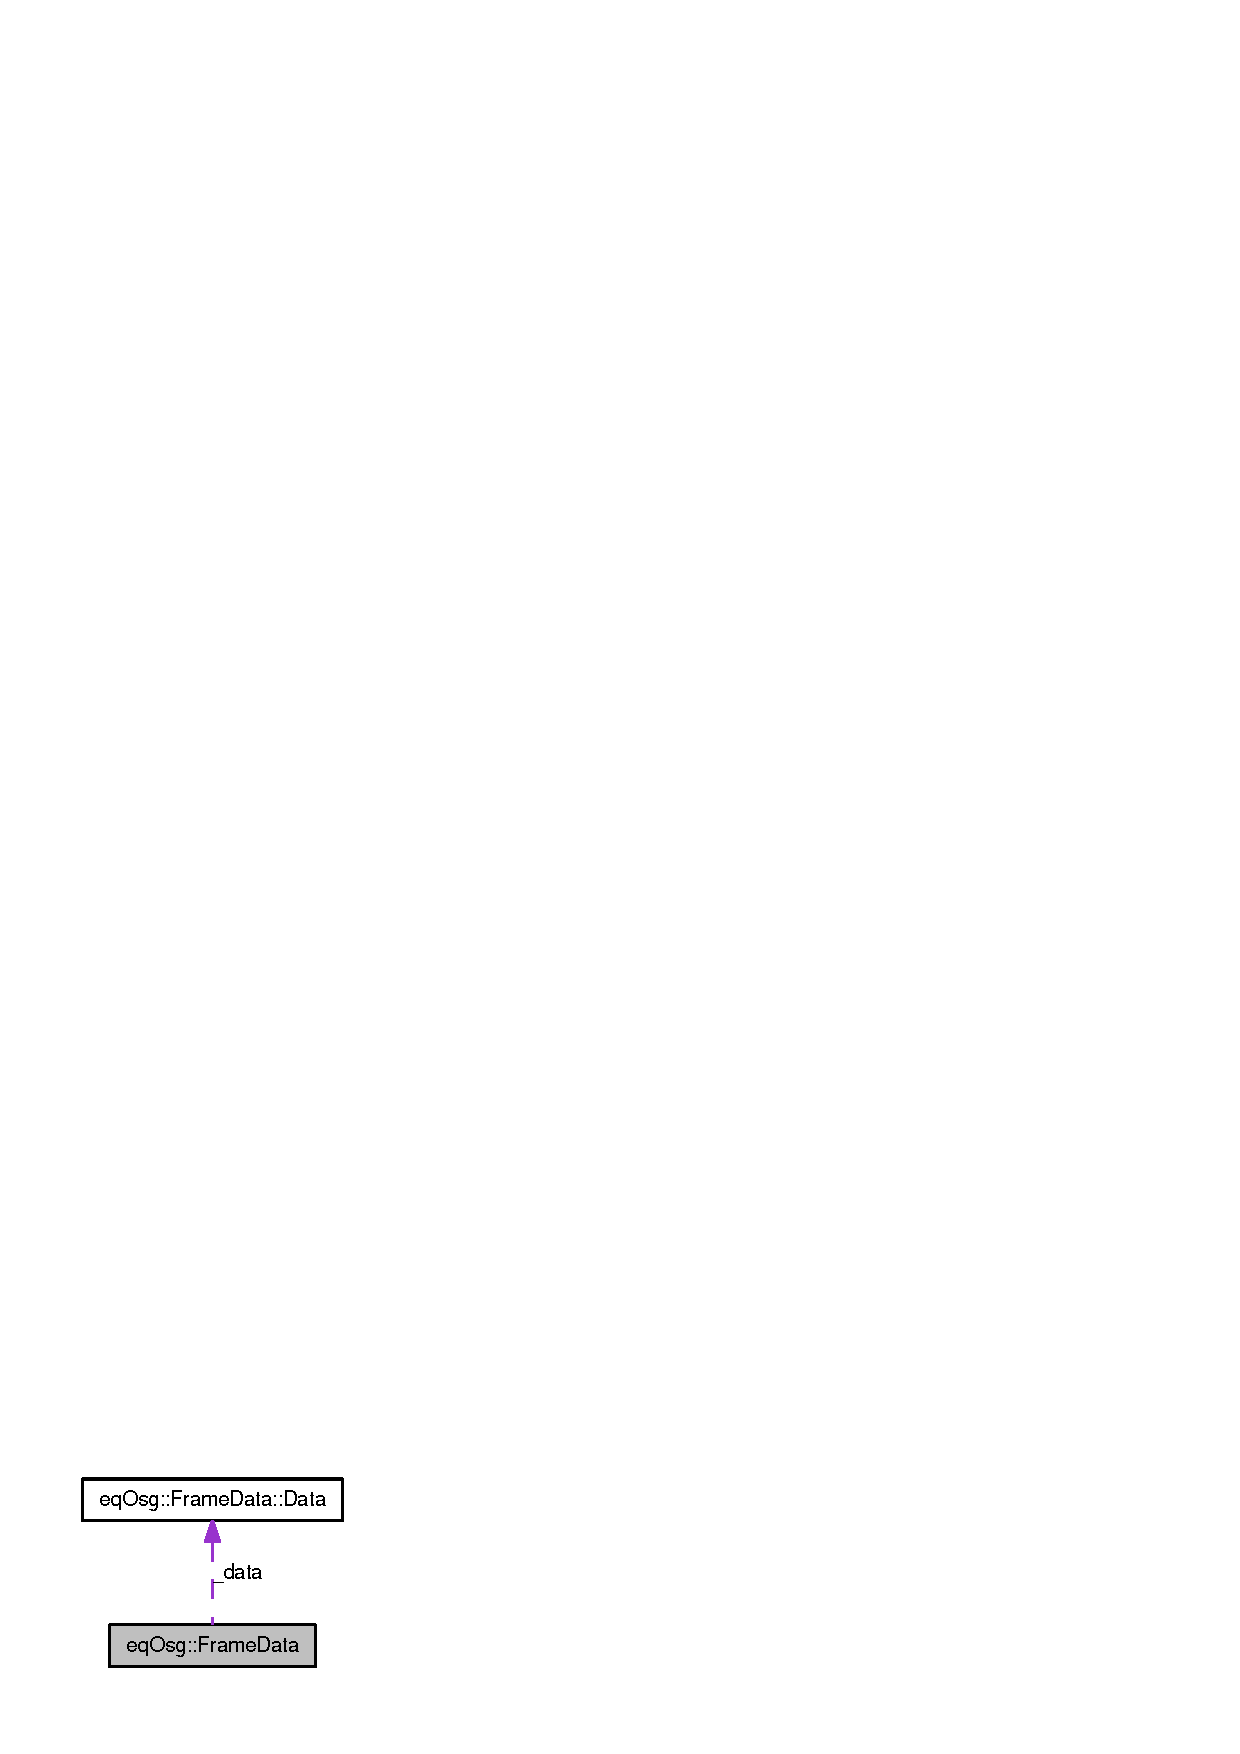
\includegraphics[width=168pt]{a00094}
\end{center}
\end{figure}
\subsection*{Classes}
\begin{CompactItemize}
\item 
struct \hyperlink{a00008}{Data}
\begin{CompactList}\small\item\em The FrameData's struct to hold members. \item\end{CompactList}\end{CompactItemize}
\subsection*{Public Member Functions}
\begin{CompactItemize}
\item 
\hyperlink{a00010_25212bee682363205562fae39028c3d6}{FrameData} ()
\begin{CompactList}\small\item\em Initialises everything to zero. \item\end{CompactList}\end{CompactItemize}
\subsection*{Public Attributes}
\begin{CompactItemize}
\item 
\hypertarget{a00010_bb269cc113e09a51c17d8d7400c6f1bb}{
\hyperlink{a00008}{Data} \hyperlink{a00010_bb269cc113e09a51c17d8d7400c6f1bb}{\_\-data}}
\label{a00010_bb269cc113e09a51c17d8d7400c6f1bb}

\begin{CompactList}\small\item\em our data struct \item\end{CompactList}\item 
\hypertarget{a00010_11589a99465896a1c632509c463c1577}{
std::vector$<$ eq::Event $>$ \hyperlink{a00010_11589a99465896a1c632509c463c1577}{\_\-eventQueue}}
\label{a00010_11589a99465896a1c632509c463c1577}

\begin{CompactList}\small\item\em save the eq events to pass it to the pipe \item\end{CompactList}\end{CompactItemize}
\subsection*{Protected Member Functions}
\begin{CompactItemize}
\item 
virtual eq::net::Object::ChangeType \hyperlink{a00010_00b26118522849f58fcc66b140a1c005}{getChangeType} () const 
\begin{CompactList}\small\item\em Change type is set to INSTANCE. \item\end{CompactList}\item 
virtual void \hyperlink{a00010_67d459f6a98840d88b1a0955aa4f517e}{getInstanceData} (eq::net::DataOStream \&stream)
\begin{CompactList}\small\item\em Passes the FrameData's data to the stream. \item\end{CompactList}\item 
virtual void \hyperlink{a00010_2dc720c76b371a3bd5edba7020808542}{applyInstanceData} (eq::net::DataIStream \&stream)
\begin{CompactList}\small\item\em Gets the data out of the stream. \item\end{CompactList}\end{CompactItemize}


\subsection{Detailed Description}
\hyperlink{a00010}{FrameData} holds all data which is updated each frame. 

It is sent by the server to all render clients. 

\subsection{Constructor \& Destructor Documentation}
\hypertarget{a00010_25212bee682363205562fae39028c3d6}{
\index{eqOsg::FrameData@{eqOsg::FrameData}!FrameData@{FrameData}}
\index{FrameData@{FrameData}!eqOsg::FrameData@{eqOsg::FrameData}}
\subsubsection[{FrameData}]{\setlength{\rightskip}{0pt plus 5cm}FrameData::FrameData ()}}
\label{a00010_25212bee682363205562fae39028c3d6}


Initialises everything to zero. 



camera base setup 

\subsection{Member Function Documentation}
\hypertarget{a00010_2dc720c76b371a3bd5edba7020808542}{
\index{eqOsg::FrameData@{eqOsg::FrameData}!applyInstanceData@{applyInstanceData}}
\index{applyInstanceData@{applyInstanceData}!eqOsg::FrameData@{eqOsg::FrameData}}
\subsubsection[{applyInstanceData}]{\setlength{\rightskip}{0pt plus 5cm}void FrameData::applyInstanceData (eq::net::DataIStream \& {\em stream})\hspace{0.3cm}{\tt  \mbox{[}protected, virtual\mbox{]}}}}
\label{a00010_2dc720c76b371a3bd5edba7020808542}


Gets the data out of the stream. 

\begin{Desc}
\item[Parameters:]
\begin{description}
\item[{\em stream}]The Equalizer stream to read. \end{description}
\end{Desc}


get the framedata out of the stream \hypertarget{a00010_00b26118522849f58fcc66b140a1c005}{
\index{eqOsg::FrameData@{eqOsg::FrameData}!getChangeType@{getChangeType}}
\index{getChangeType@{getChangeType}!eqOsg::FrameData@{eqOsg::FrameData}}
\subsubsection[{getChangeType}]{\setlength{\rightskip}{0pt plus 5cm}eq::net::Object::ChangeType FrameData::getChangeType () const\hspace{0.3cm}{\tt  \mbox{[}protected, virtual\mbox{]}}}}
\label{a00010_00b26118522849f58fcc66b140a1c005}


Change type is set to INSTANCE. 

\begin{Desc}
\item[Returns:]The Equalizer change type. \end{Desc}
\hypertarget{a00010_67d459f6a98840d88b1a0955aa4f517e}{
\index{eqOsg::FrameData@{eqOsg::FrameData}!getInstanceData@{getInstanceData}}
\index{getInstanceData@{getInstanceData}!eqOsg::FrameData@{eqOsg::FrameData}}
\subsubsection[{getInstanceData}]{\setlength{\rightskip}{0pt plus 5cm}void FrameData::getInstanceData (eq::net::DataOStream \& {\em stream})\hspace{0.3cm}{\tt  \mbox{[}protected, virtual\mbox{]}}}}
\label{a00010_67d459f6a98840d88b1a0955aa4f517e}


Passes the FrameData's data to the stream. 

\begin{Desc}
\item[Parameters:]
\begin{description}
\item[{\em stream}]The Equalizer stream to write. \end{description}
\end{Desc}


write the framedata to the stream 

The documentation for this class was generated from the following files:\begin{CompactItemize}
\item 
E:/schule/Thesis/Repo/trunk/crf/src/FrameData.h\item 
E:/schule/Thesis/Repo/trunk/crf/src/FrameData.cpp\end{CompactItemize}
